\chapter{Results}
\label{chp:results}

This chapter reports the results in the order of the experiments in
Chapter~\ref{chp:experiments}. Section~\ref{sec:res_discovery} compares
the discovered control-flow models (E1). Section~\ref{sec:res_rules}
audits the selected model against the domain rules and evaluates its
repair (E2). Section~\ref{sec:res_baseline} executes the candidates in
ProSiT and compares the generated visits with the validation log (E3).
Each section ends with a short conclusion that states what the evidence
supports and what it does not.

% Structure for every experiment: question -> result -> explanation ->
% bounded conclusion. Unsuccessful variants are reported as well.

%%%%%%%%%%%%%%%%%%%%%%%%%%%%%%%%%%%%%%%%%%%%%%%%%%%%%%%%%%%%%%
\section{Discovery Comparison and Model Choice (E1)}
\label{sec:res_discovery}
%%%%%%%%%%%%%%%%%%%%%%%%%%%%%%%%%%%%%%%%%%%%%%%%%%%%%%%%%%%%%%
% Sources (trucksimulation repository):
%   nets: data/processed/CTB/Full Log ProM Petri Nets (ProM Lite 1.4, discovered on
%         xes_files/full_train_prom_no_nan.xes)
%   metrics: process_discovery/evaluate_prom_nets.py --log-set full
%            -> process_discovery/outputs/runs/prom_nets_full_20261102 (SUMMARY.md, conformance_overview.csv)
%   figure: process_discovery/plot_e1_tradeoff.py
%   ILP nets: prom_nets_full_ilp_20261103; prefix reference: build_prefix_reference.py
%         -> data/processed/CTB/Reference Nets, evaluated in prom_nets_full_prefix_20261103
%   ProM/PM4Py cross-check: process_discovery/outputs/runs/prom_nets_20261102 (restricted logs)
%   ProM precision plugin: process_discovery/prom_precision.py re-implements
%         PNetAlignmentAnalysis 6.10.114 AlignmentPrecGen (source in the jar)
%         -> prom_nets_full_20261102/prom_precision_train.csv (also per-sequence ETC: pm4py_etc_variants)

The eighteen nets of Table~\ref{tab:exp_grid} were discovered in ProM on the
training partition of the expanded population (58,262 visits, 80 distinct
activity sequences). They were evaluated with PM4Py as described in
Section~\ref{sec:exp_discovery_eval} on the training partition and on the
validation partition (14,625 visits, 59 sequences, six of which never occur in
training).

ProM's own replayer serves as a cross-check of the alignments. It was run on
the validation partition for the five Inductive Miner nets with the standard
cost function and penalised improper completion, using the splitting replayer,
an A$^*$ search that guarantees optimal alignments and is the default of ProM's
replay plugin \cite{vanDongen2018Splitting,vanDongen2018Datastructures}
(Table~\ref{tab:res_prom_replay}). ProM and PM4Py return the same number of
fitting visits and the same total deviation cost for every net, and the same
mean trace fitness to the two decimals that ProM reports. They differ only in
how equally cheap deviations are split between log and model moves, and in the
number of silent moves, which cost nothing in ProM.
% ProM values: "Replay a Log on Petri Net for Conformance Analysis" (PNetReplayer 6.9.179),
% full validation log on the full-population IM nets, 2026-11-03 (screenshots of the user).
% Wizard: "Measuring fitness", improper completion penalised: yes, algorithm "Splitting replayer
% assuming at most 127 tokens in each place" (Alignment package 6.10.122, IterativeAStarPlugin).

\begin{table}[htbp]
\centering
\small
\begin{tabularx}{\textwidth}{YL{1.3cm}L{1.15cm}L{1.75cm}L{1.75cm}L{1.25cm}L{1.3cm}}
\toprule
& \multicolumn{2}{l}{\textbf{Fitting visits}} & \multicolumn{2}{l}{\textbf{Log / model moves}} & \textbf{Mean trace} & \textbf{Precision} \\
\textbf{Net} & \textbf{ProM} & \textbf{share} & \textbf{ProM} & \textbf{PM4Py} & \textbf{fitness} & \textbf{(PM4Py)} \\
\midrule
IM 0.0 & 14,624 & 99.99\,\% & 1 / 0 & 1 / 0 & 1.00 & 0.869 \\
IMf 0.1 & 13,535 & 92.55\,\% & 1,105 / 0 & 881 / 224 & 0.99 & 0.914 \\
IMf 0.2 & 13,667 & 93.45\,\% & 966 / 0 & 742 / 224 & 0.99 & 0.896 \\
IMf 0.3 & 13,897 & 95.02\,\% & 735 / 0 & 735 / 0 & 0.99 & 0.900 \\
IMf 0.4 & 9,249 & 63.24\,\% & 1,181 / 4,730 & 1,177 / 4,734 & 0.93 & 0.973 \\
\bottomrule
\end{tabularx}
\caption{ProM replay of the validation partition (14,625 visits) on the five
Inductive Miner nets. PM4Py returns the same number of fitting visits and the
same total deviation cost (log plus model moves) for every net. Mean trace
fitness as reported by ProM. The last column adds the PM4Py precision: the
filtered nets reject 5.0 to 7.5\,\% of the visits for at most 0.045 more
precision, and IMf 0.4 rejects more than a third.}
\label{tab:res_prom_replay}
\end{table}

ProM's precision plugins compute measures that differ from the
escaping-edges precision used here. \emph{Measure Precision/Generalization}
(package PNetAlignmentAnalysis) reports lower values: 0.664 instead of 0.897
for IMf 0.2 on the training partition. By
default, the plugin counts every distinct sequence once and averages a ratio
per event. It also counts an activity as enabled if it becomes enabled after
silent transitions are fired backwards, provided their output places are
marked, whether or not they occurred in the trace. This re-opens choices that
the visit has already passed. Before \texttt{Gate Out}, for example, IMf 0.2
is credited with ten enabled activities instead of one. This step penalises
silent transitions rather than additional behaviour. The precision of the
Multi-perspective Process Explorer \cite{Mannhardt2016Precision} weights by
frequency and has no backward step, but it treats every silent transition as
a step of its own. It reports 0.958 for IMf 0.2 and 0.612 for IM 0.0. For
IM 0.0, the value depends on the alignment: the same measure, computed on two
other optimal alignments that contain the same 749,230 moves in a different
order, gives 0.534 and 0.394. In nets with silent transitions in concurrent
branches, this measure therefore reflects where the alignment places the
silent moves rather than the behaviour of the net. The escaping-edges
precision avoids both effects because it compares visible activities only.
All precision values in this thesis are computed with PM4Py, and values of
different tools are not mixed.
% MPE values: ProM Lite 1.4, Multi-perspective Process Explorer, precision mode,
% full training log (179,970 events), 2026-11-03. IM 0.0: 1,705,595 moves observed,
% 2,788,292 possible. Alternative alignments: prom_precision.py (dpn_precision) with
% PM4Py state-equation A* and Dijkstra (less memory).
% ProM value: Measure Precision/Generalization (PNetAlignmentAnalysis 6.10.114, default
% "one trace class per sequence" ticked) on the full-population IMf 0.2 net with the
% alignment on the full training log, 2026-11-03: precision 0.664, generalization 0.995.
% Re-implementation in prom_precision.py: precision 0.633 to 0.667 depending on which
% equally cheap alignment is chosen for non-fitting sequences, generalization 0.995.

\subsection{Overall Comparison}

Table~\ref{tab:res_grid} reports soundness, size, fitness and precision.
Figure~\ref{fig:res_tradeoff} places every net in the plane of fitting
validation visits and validation precision.

\begin{table}[htbp]
\centering
\small
\begin{tabularx}{\textwidth}{YL{0.8cm}L{1.9cm}L{1.15cm}L{1.15cm}L{1.15cm}L{1.15cm}L{1.15cm}}
\toprule
& & & \multicolumn{2}{l}{\textbf{Fitting visits}} & \textbf{Fitness} & \multicolumn{2}{l}{\textbf{Precision}} \\
\textbf{Net} & \textbf{Sound} & \textbf{Places / trans. (silent)} & \textbf{train} & \textbf{val.} & \textbf{val.} & \textbf{train} & \textbf{val.} \\
\midrule
IM 0.0 & yes & 28 / 38 (27) & 100\,\% & 99.99\,\% & 0.9998 & 0.903 & 0.869 \\
IMf 0.1 & yes & 10 / 17 (6) & 95.07\,\% & 92.55\,\% & 0.9851 & 0.914 & 0.914 \\
IMf 0.2 & yes & 7 / 15 (4) & 95.58\,\% & 93.45\,\% & 0.9870 & 0.897 & 0.896 \\
IMf 0.3 & yes & 11 / 18 (7) & 96.51\,\% & 95.02\,\% & 0.9901 & 0.906 & 0.900 \\
IMf 0.4 & yes & 11 / 17 (6) & 68.48\,\% & 63.24\,\% & 0.9338 & 0.982 & 0.973 \\
\midrule
HM 0.7 & yes & 22 / 45 (34) & 99.45\,\% & 99.02\,\% & 0.9983 & 0.998 & 0.994 \\
HM 0.8 & yes & 22 / 42 (31) & 98.34\,\% & 97.69\,\% & 0.9961 & 0.999 & 0.997 \\
HM 0.9 & yes & 22 / 37 (26) & 97.98\,\% & 97.29\,\% & 0.9955 & 1.000 & 0.998 \\
HM 0.9, freq.\ 0.1 & yes & 10 / 11 (6) & 71.62\,\% & 66.65\,\% & 0.9066 & 1.000 & 1.000 \\
\midrule
ILP 0.00, 0.25 & yes & 6 / 5 (2) & 40.64\,\% & 34.86\,\% & 0.7935 & 1.000 & 1.000 \\
ILP 0.55 & yes & 6 / 6 (2) & 63.84\,\% & 58.42\,\% & 0.8770 & 1.000 & 1.000 \\
ILP 0.75 & yes & 8 / 7 (2) & 78.16\,\% & 73.80\,\% & 0.9481 & 0.855 & 0.842 \\
ILP 0.95 & yes & 12 / 11 (2) & 99.05\,\% & 98.37\,\% & 0.9967 & 0.838 & 0.805 \\
ILP 1.00 & yes & 24 / 13 (2) & 100\,\% & 100\,\% & 1.0000 & 0.773 & 0.747 \\
\midrule
Prefix tree$^{b}$ & yes & 164 / 242 (80) & 100\,\% & 99.96\,\% & 0.9999 & 1.000 & 0.969 \\
\midrule
Alpha$^{a}$ & no & 4 / 11 (0) & 15.91\,\% & 16.05\,\% & 0.8625 & 0.633 & 0.612 \\
Alpha+$^{a}$ & no & 5 / 11 (0) & 15.91\,\% & 16.05\,\% & 0.8625 & 0.718 & 0.693 \\
Alpha++ & no & 22 / 11 (0) & -- & -- & -- & -- & -- \\
\bottomrule
\end{tabularx}
\caption{Discovered nets on the training partition (58,262 visits) and the
validation partition (14,625 visits). Fitting visits: share of visits whose
alignment has no deviation. Fitness: alignment-based log fitness. IM: Inductive
Miner, IMf with the noise threshold given; HM: iDHM with the dependency
threshold given; ILP: ILP Miner with the filter threshold given (0.00 and 0.25
yield the same net). $^{a}$Unsound, values reported as a diagnostic only. Alpha++
has no reachable final marking, so no alignment exists. $^{b}$Reference net that
accepts exactly the training sequences (Section~\ref{sec:exp_candidates}).}
\label{tab:res_grid}
\end{table}

None of the three Alpha nets is sound. Alpha++ cannot reach its final marking
at all, and Alpha and Alpha+ accept only 16\,\% of the visits. By the protocol
they are not executable in the simulator and are not considered further. All
Inductive Miner, Heuristics and ILP nets are sound.

Without filtering, IM 0.0 accepts every training visit and all but one
validation visit. Its validation precision is 0.869. Filtering trades this
coverage for little precision. With thresholds 0.1 to 0.3, precision rises to
at most 0.914, while 5.0 to 7.5\,\% of the validation visits are rejected. The
effect is not monotone: IMf 0.2 is less precise than IMf 0.1. At 0.4,
precision reaches 0.973, but more than a third of the visits are rejected.

The Heuristics nets reach almost perfect precision (0.994 to 0.998) and still
accept 97 to 99\,\% of the validation visits. On these two measures, HM 0.7
is better than every filtered Inductive Miner net. The net with frequency
threshold 0.1 contains only 5 of the 11 activities (the gates,
\texttt{RMG\_delivery}, \texttt{RMG\_receive} and \texttt{LL\_delivery}) and
rejects every visit with any other stop.

For the ILP Miner, a higher filter threshold keeps more behaviour. At 0.00
and 0.25 the miner returns the same net, which permits only the most frequent
sequence, \texttt{Gate In > RMG\_receive > Gate Out} (40.6\,\% of the training
visits). At 0.55 the net adds \texttt{RMG\_delivery} as an alternative stop.
These nets reach a precision of 1.000 because they permit only one or two
sequences. Without filtering, ILP 1.00 accepts every training and every
validation visit, including the visit that IM 0.0 rejects. Its validation
precision of 0.747 is the lowest among the sound nets. At 0.95, 1.6\,\% of the
validation visits are rejected, and precision rises only to 0.805.

In Figure~\ref{fig:res_tradeoff}, only ILP 1.00, IM 0.0 and the Heuristics
nets lie on the front of non-dominated nets: ILP 1.00 and IM 0.0 with the
highest fitness, the Heuristics nets with the highest precision. ILP 1.00 is
ahead of IM 0.0 by a single validation visit and behind it by 0.122 in
precision.

The prefix tree only memorises the 80 training sequences. It accepts 99.96\,\%
of the validation visits and rejects exactly the six visits whose sequence
never occurs in training. Its precision is 1.000 on the training partition by
construction and 0.969 on the validation partition, where only 53 of the 80
training sequences recur. Together with ILP 1.00, it marks the range for nets
that keep every training sequence: 0.969 if nothing else is permitted, 0.747 if
every sequence of stops is permitted. IM 0.0 lies between the two at 0.869.
The Heuristics nets are more precise than the prefix tree, which is only
possible because they reject observed sequences.

For all sound nets with more than 90\,\% fitting visits, the share of fitting
visits drops by at most 2.6 percentage points from training to validation. The
validation period contains few new sequences: 53 of its 59 sequences also
occur in training.

\begin{figure}[htbp]
\centering
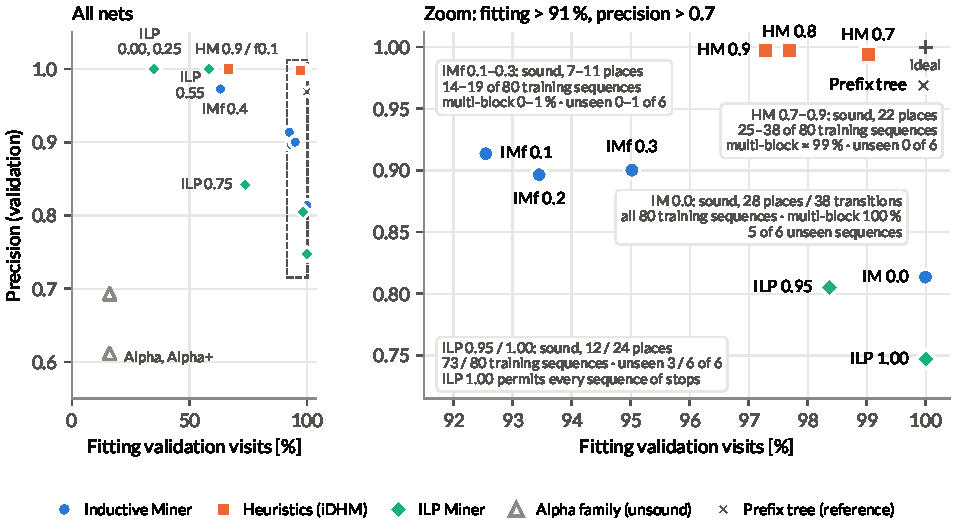
\includegraphics[width=\textwidth]{figures/discovery_prom/e1_fitness_precision.pdf}
\caption{Fitness--precision trade-off of the discovered nets on the validation
partition. Left: all nets with an alignment; the dashed rectangle marks the
zoomed region. Right: the candidates with more than 91\,\% fitting visits.
Boxes summarise soundness, size and the coverage measures of
Table~\ref{tab:res_coverage}. Hollow grey markers: the unsound Alpha nets.
The prefix tree is a reference, not a candidate.}
\label{fig:res_tradeoff}
\end{figure}

\subsection{What the Aggregate Measures Hide}

The share of fitting visits weights each sequence by its frequency. A net can
therefore reject many observed sequences and still fit 99\,\% of the visits.
Table~\ref{tab:res_coverage} counts the distinct sequences that each net
accepts and the acceptance of multi-block visits, the visit group that the
restricted population had excluded (Section~\ref{sec:exp_discovery_input}).

\begin{table}[htbp]
\centering
\small
\begin{tabularx}{\textwidth}{YL{1.9cm}L{1.9cm}L{2.1cm}L{2.4cm}}
\toprule
\textbf{Net} & \textbf{Training sequences accepted (of 80)} & \textbf{Validation sequences accepted (of 59)} & \textbf{Unseen validation sequences accepted (of 6)} & \textbf{Multi-block visits accepted, train / val.} \\
\midrule
IM 0.0 & 80 & 58 & 5 & 100 / 100\,\% \\
IMf 0.1 & 14 & 13 & 0 & 0 / 0\,\% \\
IMf 0.2 & 15 & 16 & 1 & 1.2 / 1.0\,\% \\
IMf 0.3 & 19 & 19 & 1 & 1.2 / 1.0\,\% \\
IMf 0.4 & 7 & 7 & 0 & 1.2 / 1.0\,\% \\
\midrule
HM 0.7 & 38 & 28 & 0 & 99.4 / 99.0\,\% \\
HM 0.8 & 32 & 24 & 0 & 98.9 / 98.7\,\% \\
HM 0.9 & 25 & 19 & 0 & 98.6 / 98.7\,\% \\
HM 0.9, freq.\ 0.1 & 3 & 3 & 0 & 0 / 0\,\% \\
\midrule
ILP 0.00, 0.25 & 1 & 1 & 0 & 0 / 0\,\% \\
ILP 0.55 & 2 & 2 & 0 & 0 / 0\,\% \\
ILP 0.75 & 21 & 14 & 0 & 97.6 / 98.1\,\% \\
ILP 0.95 & 73 & 50 & 3 & 100 / 100\,\% \\
ILP 1.00 & 80 & 59 & 6 & 100 / 100\,\% \\
\midrule
Prefix tree & 80 & 53 & 0 & 100 / 99.4\,\% \\
\bottomrule
\end{tabularx}
\caption{Behaviour preserved by the sound nets and the prefix-tree reference. A sequence is accepted if the
net replays it without deviation. Multi-block visits handle containers at more
than one RMG block (1,008 training and 311 validation visits).}
\label{tab:res_coverage}
\end{table}

The Heuristics nets reach their precision by excluding observed behaviour.
HM 0.7 accepts 99.45\,\% of the training visits but only 38 of the 80
training sequences. The 42 rejected sequences cover 322 visits, and all of them
contain at least two stops. Of the 13 pairs of stops that occur in both orders
in training, HM 0.7 accepts nine in one order only and four in neither order.
Examples are \texttt{RMG\_delivery > LL\_delivery} (40 visits) and
\texttt{RMG\_receive > LL\_receive} (36 visits). The Heuristics nets accept
none of the six validation sequences that are new in this period. A net of
this kind can only reproduce the most frequent order of every combination of
stops.

The filtered Inductive Miner nets lose a regular operational pattern. IMf 0.1
accepts none of the multi-block visits, IMf 0.2 to 0.4 accept about
1\,\%. The most frequent multi-block sequence,
\texttt{Gate In > RMG\_delivery > RMG\_receive > Gate Out}, is a double cycle
whose two containers are stored in different blocks (799 training visits).
With 1.7\,\% of the training visits, the multi-block group falls below every
tested noise threshold. These visits are also the longest ones, with a median
turnaround time of 50 minutes in validation against 33 minutes for visits with
one RMG block. IMf 0.1 additionally rejects the single-stop visit
\texttt{Gate In > HO2\_mixed > Gate Out} (486 training visits).

IM 0.0 keeps every training sequence and every multi-block visit, and it
accepts five of the six new validation sequences. The one rejected validation
visit, \texttt{Gate In > HO2\_mixed > RMG\_delivery > Gate Out}, follows a
sequence that never occurs in training.

ILP 1.00 keeps all observed behaviour as well, but only because it permits
every sequence of stops between \texttt{Gate In} and \texttt{Gate Out}.
Counted on its reachability graph, it accepts $9^k$ sequences with $k$ stops,
that is, 6,561 sequences with four stops. IM 0.0 accepts 2,009 sequences with
four stops, and three occur in training. ILP 1.00 is therefore a flower model
for the stops. Its precision of 0.747 is the value that a net reaches when it
keeps the gates but imposes no constraint on the stops.
% Source: process_discovery/count_language.py -> prom_nets_full_ilp_20261103/language_counts.json
% (k = 0..4 stops: IM 0.0 1/9/61/365/2009; ILP 1.00 1/9/81/729/6561; training 0/9/38/30/3).

Precision is weighted by frequency as well. On the training partition, IM 0.0
is as precise as the filtered nets when weighted by visits (0.903 against 0.897
to 0.914). With every training sequence counted once, its precision falls to
0.665, while IMf 0.1 to 0.3 reach 0.874 to 0.895 and the Heuristics nets 0.970
to 0.989. The additional behaviour of IM 0.0 is therefore concentrated in the
rare sequences with several stops. The filtered nets are not penalised in the
same way for the sequences they reject, because these enter the measure only
through their alignments.

\subsection{The Selected Net}

Figure~\ref{fig:res_im0} shows IM 0.0. After \texttt{Gate In} and an optional
\texttt{LL\_mixed}, a silent AND-split opens five branches: \texttt{RMG\_mixed},
\texttt{RMG\_receive}, \texttt{RMG\_delivery}, a choice between
\texttt{LL\_receive} and \texttt{LL\_delivery}, and a choice between
\texttt{HO2\_receive} and \texttt{HO2\_delivery}. An optional
\texttt{HO2\_mixed} follows the last three branches. Every branch can be
skipped, and all activities except the LL activities can be repeated through
silent loops. The parallel operators express that the order of the stops is
free. Two consequences follow directly from the structure. The net permits the
visit \texttt{Gate In > Gate Out} without any handling, and it permits any
number of stops, for example five consecutive \texttt{RMG\_delivery} events.
Neither occurs in the data. These are the additional behaviour behind the
precision of 0.869, and they are examined in E2.

\begin{figure}[htbp]
\centering
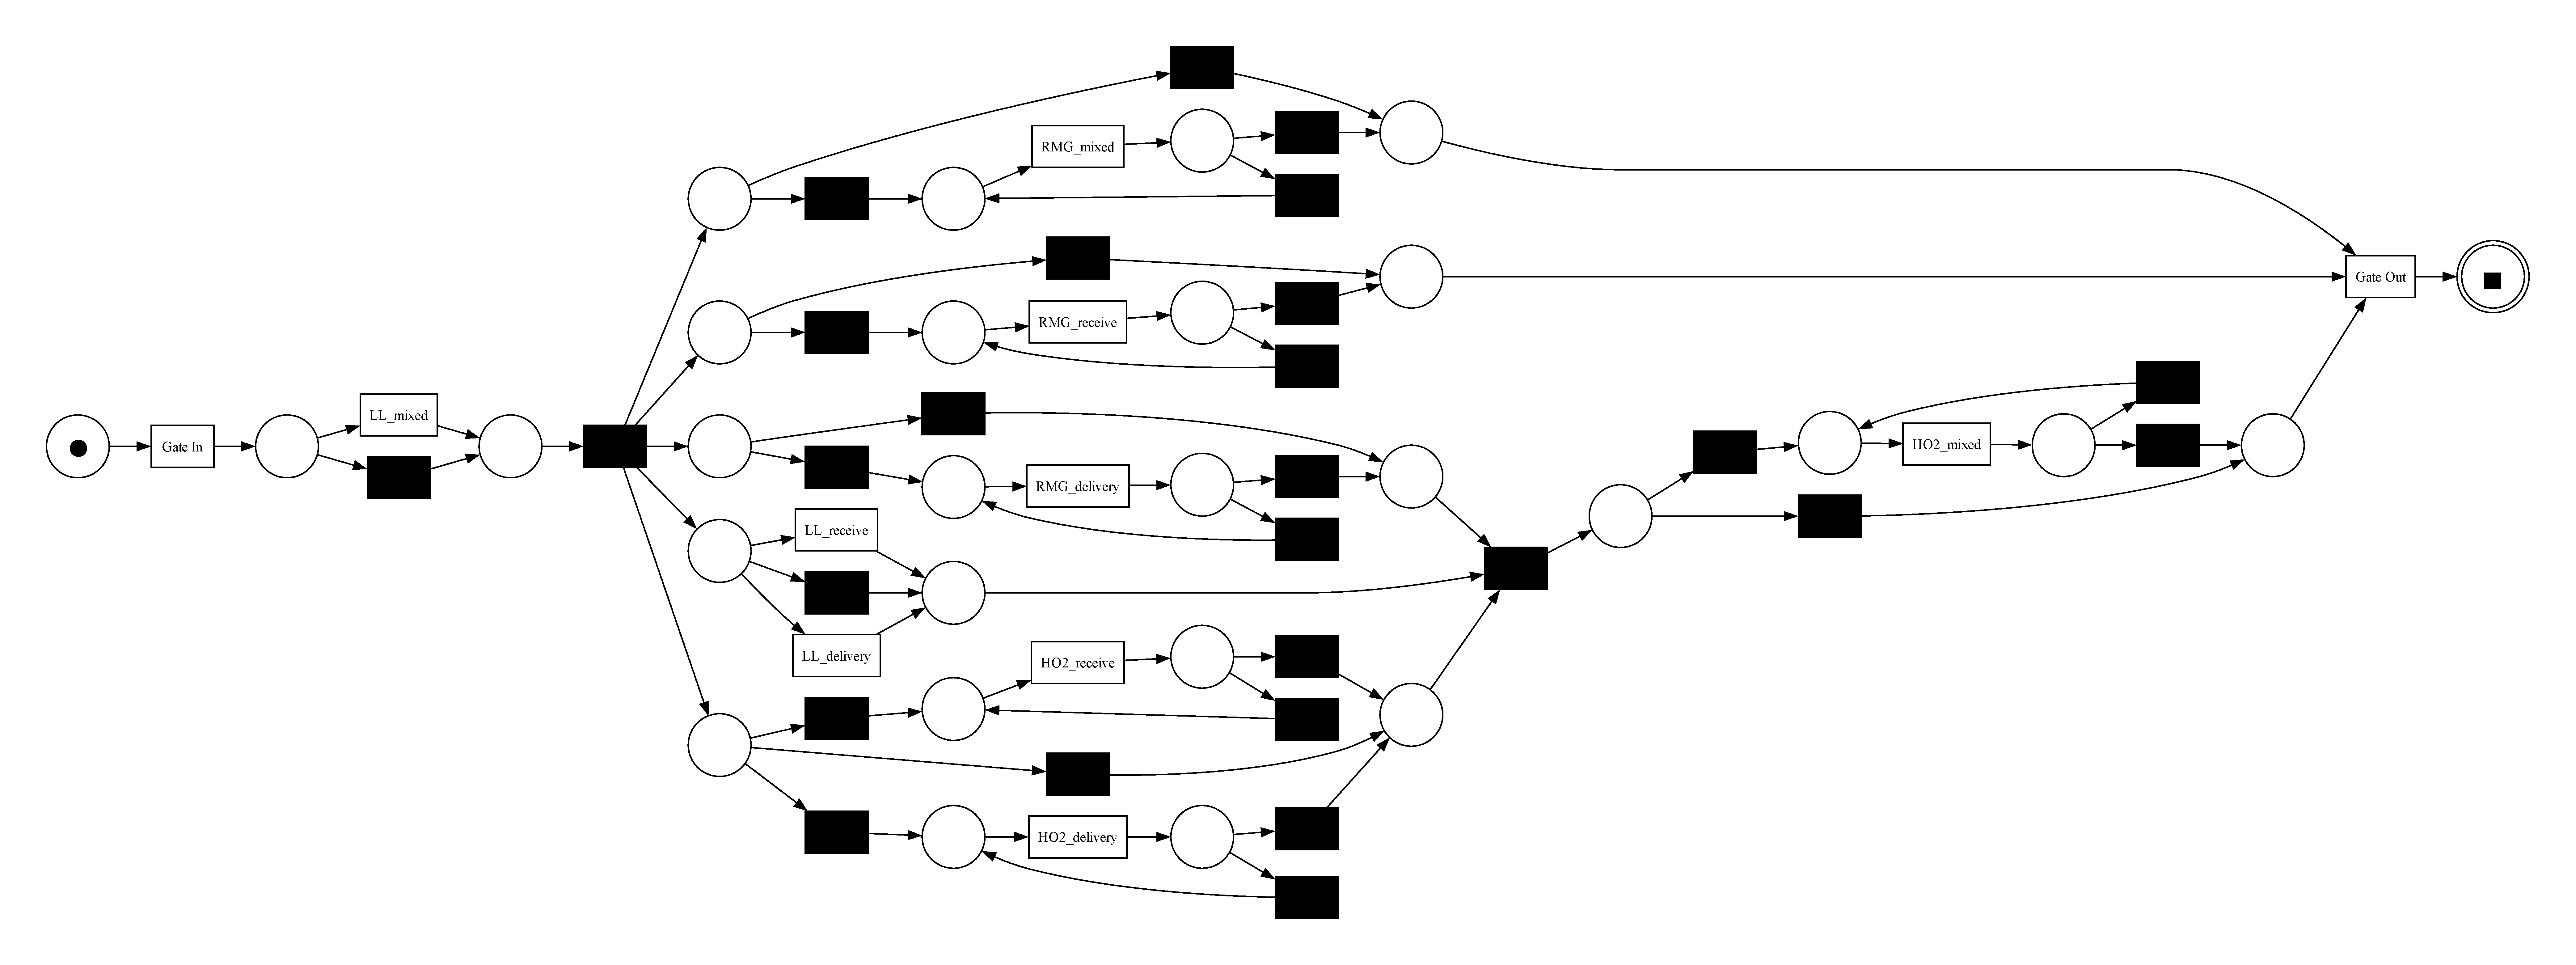
\includegraphics[width=\textwidth]{figures/discovery_prom/im00_full.pdf}
\caption{Selected net IM 0.0 (Inductive Miner without filtering, discovered in
ProM on the full training partition): 28 places, 11 visible and 27 silent
transitions (black). The silent AND-split after \texttt{Gate In} lets the
branches occur in any order. Every branch can be skipped.}
\label{fig:res_im0}
\end{figure}

\subsection{Conclusion of E1}

Two sound nets preserve all observed behaviour, that is, every training
sequence and every visit group including the multi-block visits: IM 0.0 and
ILP 1.00. ILP 1.00 does so by permitting every sequence of stops, so its
precision is that of a flower model for the stops. IM 0.0 restricts the order
and repetition of the stops (2,009 instead of 6,561 sequences with four
stops), is clearly more precise (0.869 against 0.747) and rejects a single
validation visit, whose sequence never occurs in training. IM 0.0 is retained
for E2. All other candidates obtain their higher precision by rejecting
observed behaviour. Noise filtering in IMf and ILP removes rare but regular
visit types first, and the Heuristics nets restrict most combinations of
stops to a single order. For a
simulation model this matters more than the aggregate scores suggest: a
sequence that the net rejects can never be generated.

E1 does not show that IM 0.0 is a good simulation model. Its precision of
0.869 reflects behaviour that the data do not contain, including visits
without handling and unbounded repetitions. The results also concern the
tested configurations only, not the algorithm families in general. Finally,
the comparison depends on the population. On the restricted population
without multi-block visits, the loss of this visit group by the filtered nets
would not have been visible.

%%%%%%%%%%%%%%%%%%%%%%%%%%%%%%%%%%%%%%%%%%%%%%%%%%%%%%%%%%%%%%
\section{Domain-Rule Audit and Repair (E2)}
\label{sec:res_rules}
egin{hints}
\item OUTDATED (PM4Py era, single base model IM0, rule names R1--R12). Rewrite with the E2 run on the five E1 candidates (process\_discovery/outputs/runs/e2\_top5\_20261104) and the rule numbers 1--7 of Table~
ef{tab:domain_rules}.
\end{hints}
%%%%%%%%%%%%%%%%%%%%%%%%%%%%%%%%%%%%%%%%%%%%%%%%%%%%%%%%%%%%%%

\subsection{Recorded Log}

All 58,262 training visits and all 14,625 validation visits satisfy R1
to R5, R7, R11 and R12. The largest observed visit has four yard events.
In the 5,090 training visits with at least two stops, no two stop
intervals overlap, and start and completion times increase strictly. The
gate events and the stop aggregation were constructed upstream.
Conformance of the recorded log can therefore partly follow from that
construction and is not independent evidence for the rules.

Repeated mixed events at the same unit occur in a few visits, for
example \texttt{RMG\_mixed} twice at block T19 in eight training visits
and \texttt{HO2\_mixed} twice in six. They are not counted as violations
of R12, because it is not clear whether they are two separate approaches
or an artefact of the stop reconstruction.

\subsection{Model Language}

Table~\ref{tab:res_rule_audit} shows which rules the discovered nets
violate. All sound nets satisfy the gate rules R1 to R4 by construction.
R5 is violated by IM0, IMf 0.1 and ILP 1.0. In each case, the shortest
counterexample is the visit \texttt{Gate In > Gate Out} without any
handling. None of the counterexamples occurs in the training log.

\begin{table}[htbp]
\centering
\begin{tabularx}{\textwidth}{YL{2.0cm}L{4.2cm}L{2.2cm}}
\toprule
\textbf{Net (expanded)} & \textbf{R1--R4} & \textbf{R5} & \textbf{R7} \\
\midrule
IM0 & satisfied & violated (\texttt{Gate In > Gate Out}) & unbounded \\
IMf 0.1 & satisfied & violated (\texttt{Gate In > Gate Out}) & unbounded \\
IMf 0.2 & satisfied & satisfied & unbounded \\
ILP 1.0 & satisfied & violated (\texttt{Gate In > Gate Out}) & unbounded \\
Prefix reference & satisfied & satisfied & satisfied \\
\bottomrule
\end{tabularx}
\caption{Rule audit of the model languages. ``Unbounded'' means that
loops allow arbitrarily many yard events.}
\label{tab:res_rule_audit}
\end{table}

The empty visit is not the only additional behaviour.
Table~\ref{tab:res_language} counts the distinct sequences that each net
permits, by the number of yard events. With one yard event, IM0 permits
exactly the nine observed sequences. With two yard events, it permits 61
sequences, of which 38 are observed. With four, it permits 2,009 against
3 observed. Examples of permitted but unobserved two-stop sequences are
\texttt{RMG\_mixed > RMG\_delivery} and \texttt{LL\_mixed > LL\_receive}.
Both contradict R12 when the two events take place at the same unit.

\begin{table}[htbp]
\centering
\begin{tabularx}{\textwidth}{YL{1.4cm}L{1.4cm}L{1.4cm}L{1.4cm}}
\toprule
\textbf{Yard events per visit} & \textbf{1} & \textbf{2} & \textbf{3} & \textbf{4} \\
\midrule
Observed training sequences & 9 & 38 & 30 & 3 \\
IM0 & 9 & 61 & 365 & 2,009 \\
IM0 + R5 + R12 (repaired) & 9 & 57 & 313 & 1,583 \\
ILP 1.0 & 9 & 81 & 729 & 6,561 \\
\bottomrule
\end{tabularx}
\caption{Number of distinct sequences permitted by each net, by number
of yard events. IM0 additionally permits the empty visit.}
\label{tab:res_language}
\end{table}

The parallel operators of IM0 express that the order of stops is free.
They do not mean that a truck is at two places at once. The R11 check
in the recorded log supports this reading. Whether the simulator
respects it is examined in Section~\ref{sec:res_baseline}.

\subsection{Mechanism in the Simulator}

The language audit shows what IM0 permits, not how often the simulator
will generate it. Inspection of the ProSiT 1.0.3 source code identified
two mechanisms that turn the structure of IM0 into empty visits and
overlapping stops.

The first mechanism concerns parallel branches. ProSiT enables a
transition at the latest timestamp among its input places. After an
AND-split, all branches therefore receive the same enabling time. The
second stop of a visit does not wait for the first to finish, and both
are scheduled concurrently. This violates R11.

The second mechanism concerns empty visits. IM0 reaches the empty visit
through a sequence of silent skip transitions. ProSiT learns a separate
routing model for each transition and draws each skip decision
independently. The product of several moderately likely skips gives the
empty path a substantial probability, although it never occurs in the
training data. Both effects shorten the simulated turnaround time.

\subsection{Repair}

Table~\ref{tab:res_repair} reports the repaired models. All variants
are sound and accept all 80 observed training sequences. The share of
fitting validation visits is identical for all of them.

\begin{table}[htbp]
\centering
\begin{tabularx}{\textwidth}{YL{1.9cm}L{1.9cm}L{1.6cm}L{1.6cm}L{1.6cm}}
\toprule
& \textbf{IM0} & \textbf{Control (same language)} & \textbf{+ R5} & \textbf{+ R5, R12} & \textbf{+ R5, R12, R7} \\
\midrule
Places / transitions (silent) & 32 / 46 (35) & 10 / 59 (0) & 10 / 58 (0) & 10 / 54 (0) & 51 / 309 (0) \\
Fitting validation visits & 99.993\,\% & 99.993\,\% & 99.993\,\% & 99.993\,\% & 99.993\,\% \\
Precision, validation & 0.8131 & 0.8136 & 0.8559 & 0.8644 & 0.8644 \\
Precision, training & 0.8383 & 0.8386 & 0.8823 & 0.8886 & -- \\
R5 satisfied & no & no & yes & yes & yes \\
Concurrent stops possible & yes & no & no & no & no \\
\bottomrule
\end{tabularx}
\caption{Repaired variants of IM0 on the expanded population. The
control encodes the unrestricted IM0 language as a state machine.}
\label{tab:res_repair}
\end{table}

The control isolates the effect of the representation. Encoding the same
language as a state machine changes precision by only 0.0005. The gain
of 0.043 from R5 therefore comes from removing the empty visit. After
Gate In, Gate Out had always been a permitted continuation that the log
never uses. R12 adds another 0.008 by excluding the four unobserved
two-stop sequences that combine a mixed event with a separate delivery
or receive at LL or HO2. The upper bound of eight yard events (R7)
changes no metric, because no observed visit exceeds four. It enlarges
the net from 54 to 309 transitions and adds transitions for five to
eight stops that have no training data. R7 is therefore not used in the
simulation.

The slightly higher fitness of the state machines (0.99999 against
0.99976) is a cost artefact of the silent transitions in IM0. The set of
accepted visits is the same.

The repaired net (Figure~\ref{fig:res_repaired}) still permits 19
unobserved two-stop sequences, for example
\texttt{RMG\_delivery > RMG\_mixed}. They are excluded neither by the
data nor by a confirmed rule. Under the generic labels they are
admissible when the two events take place at different blocks.
% TODO: list of the 19 sequences in the appendix, with the terminal's
% assessment from the questionnaire (part B3).

\begin{figure}[htbp]
\centering
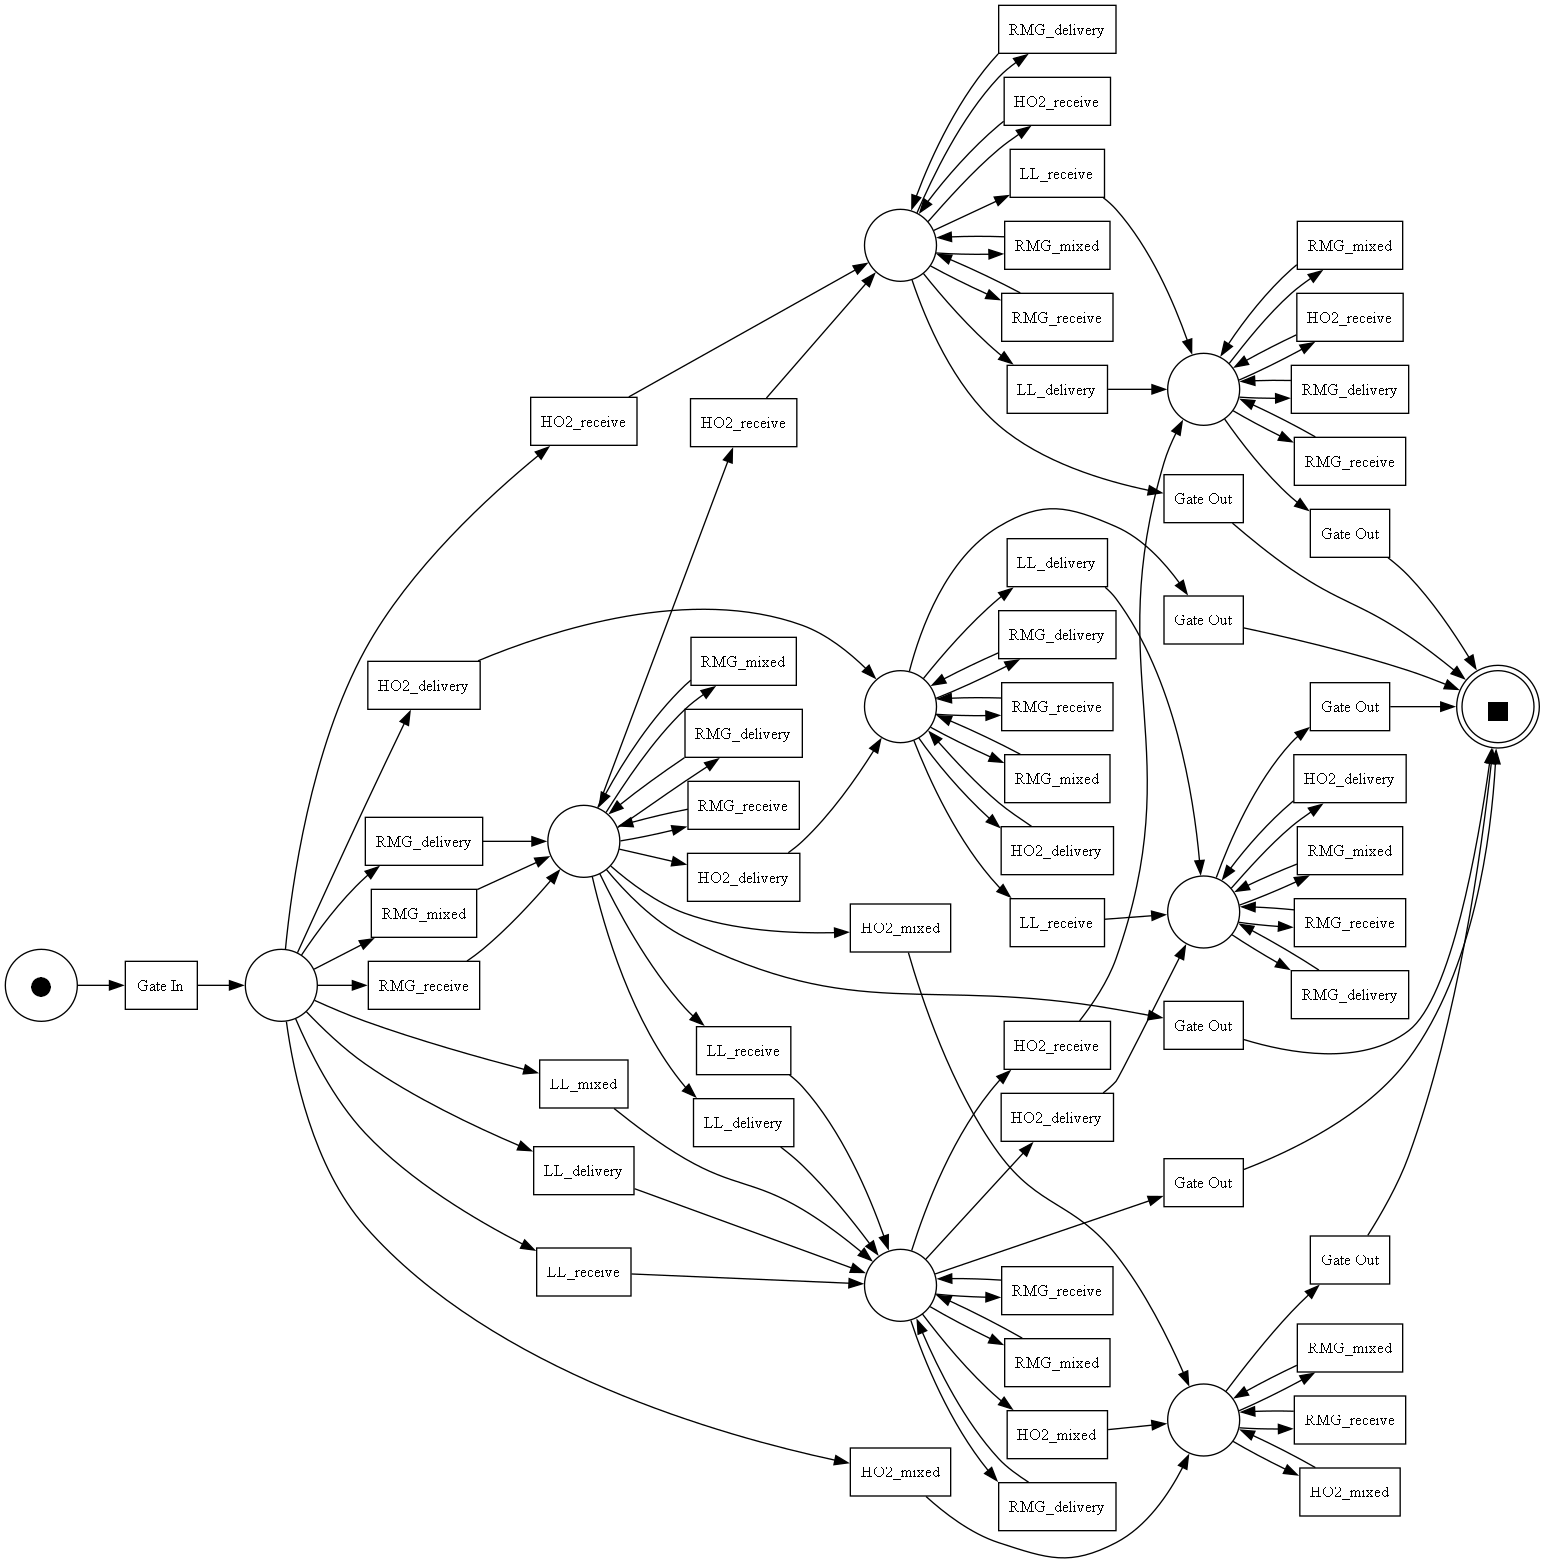
\includegraphics[width=\textwidth]{figures/discovery_2026/im0_r5_r12_state_machine.png}
\caption{Repaired control-flow model \texttt{IM0\_R5\_R12} as a state
machine (10 places, 54 transitions). Each place is a state of the visit.
Repeated labels belong to different states.}
\label{fig:res_repaired}
\end{figure}

\subsection{Contribution of the Base Model}

The restricted model is the language of the base model intersected with
the rules. The rules can only remove behaviour. The base model therefore
decides two things: which observed sequences are already lost, and which
unobserved sequences remain. Table~\ref{tab:res_ladder} applies the same
restriction (R5 and R12) to every sound base model.

\begin{table}[htbp]
\centering
\begin{tabularx}{\textwidth}{YL{2.6cm}L{1.6cm}L{1.6cm}L{2.0cm}}
\toprule
\textbf{Base model} & \textbf{Permitted sequences, 1 / 2 / 3 / 4 yard events} & \textbf{Training sequences kept (of 80)} & \textbf{Validation visits accepted} & \textbf{Precision (validation), base $\rightarrow$ restricted} \\
\midrule
Observed training log & 9 / 38 / 30 / 3 & 80 & -- & -- \\
\midrule
Prefix reference & 9 / 38 / 30 / 3 & 80 & 99.96\,\% & 0.969 $\rightarrow$ 0.969 \\
Heuristics, no AND & 9 / 7 / 1 / 0 & 17 & 97.26\,\% & 0.9999 $\rightarrow$ 0.9999 \\
Split Miner, $\varepsilon = 0$ & 4 / 0 / 6 / 12 & 4 & 40.33\,\% & 0.938 $\rightarrow$ 0.961 \\
IMf 0.2 & 6 / 16 / 18 / 20 & 24 & 85.20\,\% & 0.999 $\rightarrow$ 0.999 \\
IMf 0.1 & 9 / 16 / 18 / 20 & 27 & 94.64\,\% & 0.927 $\rightarrow$ 0.999 \\
IM0 & 9 / 57 / 313 / 1,583 & 80 & 99.99\,\% & 0.813 $\rightarrow$ 0.864 \\
ILP, alpha 1.0 & 9 / 73 / 549 / 3,937 & 80 & 100\,\% & 0.747 $\rightarrow$ 0.800 \\
\bottomrule
\end{tabularx}
\caption{The same rule restriction (R5, R12) applied to every sound base
model. Permitted sequences are counted after the restriction. Validation
visits accepted refers to the restricted model.}
\label{tab:res_ladder}
\end{table}

Three observations follow. First, the restriction cannot restore what
the base model has already excluded. Base models that filter observed
behaviour keep only 4 to 27 of the 80 training sequences. Second, among
the base models that keep all observed sequences, the choice of base
model is a choice of how far the model generalises. The prefix reference
keeps only the observed sequences and rejects the six validation visits
whose sequence never occurs in training. The restricted IM0 accepts five
of them. The restricted ILP net accepts all of them, but permits 3,937
sequences with four yard events against three observed. Third, IM0 lies
between these extremes. It generalises to unobserved combinations of
observed stop types, at a precision of 0.864, without becoming a flower
model. Selecting IM0 is thus a choice of a moderate level of
generalisation, supported by its acceptance of new validation sequences.

\subsection{Conclusion of E2}

IM0 permits the empty visit and, through its parallel branches, allows
the simulator to schedule two stops of one truck at the same time. The
repair removes both without losing an observed sequence and raises
validation precision from 0.813 to 0.864. The remaining
overgeneralisation consists of unobserved sequences that are plausible
under the generic labels. E2 shows that the repaired model is a better
description of the permitted truck behaviour. It does not yet show that
it produces a better simulation. That is the question of E3.

%%%%%%%%%%%%%%%%%%%%%%%%%%%%%%%%%%%%%%%%%%%%%%%%%%%%%%%%%%%%%%
\section{Control-Flow Candidates in the Simulation (E3)}
\label{sec:res_baseline}
egin{hints}
\item OUTDATED (ProSiT 1.0.3, candidates CONTRACT/IM0/IM0\_R5\_R12). Rewrite with the E3 runs on ILP 1.00 repaired, IM 0.0 repaired and HM 0.7 and the $2	imes2$ contrast (simulation\_e3/runs/e3\_prom\_20261104, e3\_prom\_noguard\_20261104, e3\_prom\_guard\_original\_20261104).
\end{hints}
%%%%%%%%%%%%%%%%%%%%%%%%%%%%%%%%%%%%%%%%%%%%%%%%%%%%%%%%%%%%%%

% PROVISIONAL: values below come from the diagnostic script
% trucksimulation/analysis/critical_review_20261007/scripts/e3_provisional_kpis.py
% Replace with the outputs of the final E3 validator before submission.

Table~\ref{tab:res_e3} compares the three candidates with the validation
log. All values are means over five replications. The range across
replications is small, with at most one minute for the medians and
about one percentage point for the structural shares.

\begin{table}[htbp]
\centering
\begin{tabularx}{\textwidth}{YL{1.7cm}L{1.7cm}L{1.7cm}L{1.9cm}}
\toprule
\textbf{Measure} & \textbf{Observed} & \textbf{CONTRACT} & \textbf{IM0} & \textbf{IM0\_R5\_R12} \\
\midrule
\multicolumn{5}{l}{\textit{Visit structure}} \\
Visits without yard event & 0\,\% & 0\,\% & 15.7\,\% & 0\,\% \\
Visits with 1 / 2 / $\geq$3 stops & 89.8 / 10.1 / 0.1\,\% & 92.9 / 4.8 / 2.3\,\% & 62.6 / 16.2 / 5.5\,\% & 91.1 / 8.2 / 0.7\,\% \\
Multi-stop visits with overlapping stops & 0\,\% & 0\,\% & 71.6\,\% & 0\,\% \\
RMG visits with several blocks & 2.9\,\% & 2.9\,\% & 1.2\,\% & 2.1\,\% \\
\midrule
\multicolumn{5}{l}{\textit{Turnaround time [min]}} \\
TTT mean / median / P90 & 42.2 / 34 / 78 & 33.1 / 28 / 57 & 28.0 / 25 / 49 & 31.2 / 27 / 53 \\
Median TTT, delivery / receive / mixed & 28 / 35 / 48 & 25 / 28 / 39 & 22 / 26 / 31 & 24 / 27 / 38 \\
Mean approach / exit & 13.2 / 13.6 & 7.0 / 13.2 & 6.4 / 11.2 & 6.0 / 12.8 \\
Median stop, RMG / LL / HO2 & 9 / 7 / 12 & 8 / 7 / 9 & 8 / 7 / 10 & 8 / 7 / 9 \\
\midrule
\multicolumn{5}{l}{\textit{Load and delay peaks}} \\
Maximum arrivals per hour & 255 & 132 & 132 & 132 \\
Hours with median TTT $\geq$ 37 min & 26.4\,\% & 0\,\% & 0\,\% & 0\,\% \\
\bottomrule
\end{tabularx}
\caption{Generated visits of the three control-flow candidates compared
with the validation log. Means over five replications of 14,625 visits.
Approach is Gate In to the start of the first stop, exit is the end of
the last stop to Gate Out.}
\label{tab:res_e3}
\end{table}

\subsection{Visit Structure}

The unrepaired IM0 generates both effects predicted in E2.
15.7\,\% of its simulated visits contain no yard activity. Among its multi-stop visits, 71.6\,\% have stops that overlap
in time. Both values are zero in the recorded log. The stop distribution
is also distorted. IM0 generates too few single-stop visits and far
more visits with three or more stops than observed (5.5\,\% against
0.1\,\%).

The repaired model removes both violations completely, as the
state-machine encoding guarantees. Its stop distribution is the closest
to the observed one. The total variation distance to the observed
distribution is 0.02, against 0.05 for \texttt{CONTRACT} and 0.27 for
IM0. \texttt{CONTRACT} satisfies R5 and R11 as well, because its
structure is sequential. It generates too many visits with three or more
stops (2.3\,\% against 0.1\,\%), since its loop does not restrict how
often a yard activity is repeated.

The repaired model reproduces the stop distribution partly because its
routing trees split on the sampled case attributes \texttt{n\_stops}
and \texttt{visit\_complexity}. In 99\,\% of its simulated visits, the
number of generated stops equals the sampled \texttt{n\_stops}. For IM0
the share is 65\,\%. These attributes are part of the planned visit
manifest and are known at Gate In
(Section~\ref{sec:entry_known_attributes}). A close stop distribution
therefore shows that control flow and case attributes are consistent.
It is weaker evidence that the routing has been learned independently.

The share of RMG visits with more than one block is reproduced by
\texttt{CONTRACT} and underestimated by the repaired model (2.1\,\%
against 2.9\,\%). In the simulator the block is chosen per stop by a
learned resource model. A visit with two RMG stops may therefore be
assigned the same block twice or two different blocks. This share
depends on the resource model and not on the control flow alone. It is
examined in E4.

\subsection{Turnaround Time}

The control-flow model affects the turnaround time in the expected
direction. Removing empty visits and overlapping stops raises the median
TTT from 25 to 27 minutes and the P90 from 49 to 53 minutes. The effect
is largest for mixed visits, which often have two stops. Their median
rises from 31 minutes with IM0 to 38 minutes with the repaired model.
For IM0 a large part of the second stop is hidden by the overlap.

The effect is small compared with the remaining error. All three
candidates underestimate the observed turnaround time. The repaired
model reaches a median of 27 minutes against 34 observed, and a P90 of 53
minutes against 78. \texttt{CONTRACT} is about one minute closer in
median and P90. This is partly due to its additional long visits with
three or more stops and is therefore not evidence of a better structure.

The decomposition shows where the gap arises. Exit time and stop
durations are close to the observed values for all candidates. The
approach from Gate In to the first stop is not. Its observed mean is
13.2 minutes, the simulated means are 6.0 to 7.0 minutes. In the
repaired model, the approach accounts for about 7 of the 11 minutes
difference in mean TTT. The approach time contains the drive to the
block and the waiting before the stop starts. In ProSiT it is generated
by the waiting-time model of the first yard resource.

\subsection{Load and Delay Peaks}

None of the candidates generates a single delay-peak hour. In the
validation log, 26.4\,\% of the Gate-In hours with at least 20 visits
have a median TTT of 37 minutes or more. The arrival process explains a
large part of this difference. The simulated arrivals reach at most 132
trucks per hour, against 255 observed, and no simulated hour reaches the
arrival-peak threshold of 165. The calibrated arrival model samples
inter-arrival times from one empirical distribution and gates them only
by an on/off calendar. It reproduces the average arrival rate but not
the daily profile. Simulated arrivals are spread nearly evenly over the
day, whereas the observed arrivals concentrate between 6:00 and 18:00.
Without the load of the observed peak hours, the simulated resources do
not congest.

\subsection{Conclusion of E3}

Under identical simulation conditions, the repaired model produces
visits that respect all checked rules and reproduces the observed visit
structure most closely. The unrepaired IM0 generates empty visits and
overlapping stops at a scale that distorts the stop distribution and
the turnaround time of multi-stop visits. Discovery metrics did not
anticipate this. IM0 and the repaired model differ by 0.05 in precision
and not at all in the share of accepted visits, but by 15.7 percentage
points in simulated empty visits.

The repaired model is therefore selected as the control-flow model for
the following experiments. The comparison does not show that the
simulator reproduces the observed turnaround times. For all candidates,
the remaining error is dominated by the arrival process and the
approach time, which do not depend on the control-flow model. These two
components are the subject of E4.

%%%%%%%%%%%%%%%%%%%%%%%%%%%%%%%%%%%%%%%%%%%%%%%%%%%%%%%%%%%%%%
\section{Mechanism Audit (E4)}
\label{sec:res_mechanisms}
%%%%%%%%%%%%%%%%%%%%%%%%%%%%%%%%%%%%%%%%%%%%%%%%%%%%%%%%%%%%%%
\begin{hints}
\item Structure every subsection the same way: what was changed, result table, what the result shows, load-response test (E4b) passed or not.
\item Central table of the chapter: one row per step (E3 baseline, E4a, E4c, E4d), columns TTT median/P90, approach, delay-peak hours, Spearman hourly arrivals vs. TTT, largest block share. Sources: simulation\_e3/E4A\_ARRIVALS\_20261009.md, E4C\_BLOCKS\_CAPACITY\_20261009.md, runs/e4e\_prosit104\_20261010.
\end{hints}

\subsection{Learned Models}
\label{sec:res_inspection}
\begin{hints}
\item What ProSiT 1.0.3 learned: all execution-time models and 20 of 26 waiting-time models have a single leaf; routing splits mainly on planned visit attributes; block choice splits first on queue\_length.
\item Why: the 1.0.3 model selection compares per-leaf stability, not predictive fit. Evidence: on CTB data and on a synthetic example with clearly different groups, it always selects a single distribution; the 1.0.4 criterion selects trees.
\item What ProSiT 1.0.4 learned (tree inventory of the rediscovery). One real tree as a figure.
\end{hints}

\subsection{Arrivals (E4a)}
\label{sec:res_e4a}
\begin{hints}
\item E3 arrivals: maximum 132 trucks per hour vs. 255 observed, no arrival peaks, 14\,\% of arrivals on Saturdays.
\item Hour-of-week model reproduces the profile (67.7\,\% of arrivals between 7 and 16 h vs. 67.2\,\%); replay reproduces it exactly.
\item Result: TTT unchanged (median 27, P90 54 min), delay-peak hours 0.5--1.8\,\% vs. 26\,\%, Spearman $\approx 0$. Arrivals were necessary but not sufficient. E4b failed.
\end{hints}

\subsection{Block Choice and Capacity (E4c)}
\label{sec:res_e4c}
\begin{hints}
\item Diagnosis: block choice concentrates 29\,\% of RMG stops on one block (observed maximum 6\,\%); 79\,\% of stops start with four or more trucks at a block, because capacity is checked at enabling time.
\item With an enforced capacity, the learned block choice sends all RMG stops to one block (runaway, median TTT 15 h). Cause: the training queue length of the chosen block includes the visit's own stop.
\item With empirical or replayed block choice and capacity checked at start: block loads realistic (correlation 0.97), cap holds, but TTT and delay peaks unchanged. E4b failed.
\item Remaining cause, quantified: the waiting-time target keeps 6.2 of 11.0 minutes of observed approach time (single-server definition).
\end{hints}

\subsection{Timing Models and ProSiT Version (E4d)}
\label{sec:res_e4d}
\begin{hints}
\item Results of the ProSiT 1.0.4 rediscovery: which time models now split, on which features; simulation results of the four configurations.
\item Load-response test (E4b) on the best configuration, including arrival scaling 0.8/1.0/1.2.
\item If a load-dependent timing extension was needed: its fit to the observed curves (approach vs. block occupancy, stop duration vs. occupancy) and to the system-level behaviour that was not fitted (TTT vs. trucks in terminal, delay peaks).
\end{hints}

\subsection{Conclusion of E4}
\label{sec:res_e4_conclusion}
\begin{hints}
\item Which layers failed, why, which repairs were needed, and whether the final configuration passes the load-response test.
\item This is the answer to RQ2. State it without overclaiming: valid for turnaround time and delay peaks, not for everything.
\end{hints}

%%%%%%%%%%%%%%%%%%%%%%%%%%%%%%%%%%%%%%%%%%%%%%%%%%%%%%%%%%%%%%
\section{Final Baseline and Hold-Out Check}
\label{sec:res_holdout}
%%%%%%%%%%%%%%%%%%%%%%%%%%%%%%%%%%%%%%%%%%%%%%%%%%%%%%%%%%%%%%
\begin{hints}
\item The frozen configuration on the validation period and once on the test period, same measures, one table. No changes after seeing the test result.
\item Block congestion in the baseline: share of stops at blocks with three or more trucks, approach by block.
\end{hints}

%%%%%%%%%%%%%%%%%%%%%%%%%%%%%%%%%%%%%%%%%%%%%%%%%%%%%%%%%%%%%%
\section{Load-Aware Block Allocation (E5)}
\label{sec:res_policy}
%%%%%%%%%%%%%%%%%%%%%%%%%%%%%%%%%%%%%%%%%%%%%%%%%%%%%%%%%%%%%%
\begin{hints}
\item Only if E4b is passed. Otherwise: what the model would need to evaluate S1, and why the current evidence does not allow a quantitative statement.
\end{hints}

\subsection{Effect on the KPI}
\label{sec:res_s1_kpi}
\begin{hints}
\item Paired differences (S1 minus baseline) for the three variants $\pm 1$, $\pm 2$, any block: delay-peak hours, TTT P90 and median, with 95\,\% intervals.
\end{hints}

\subsection{Mechanism and Distribution of Effects}
\label{sec:res_s1_mechanism}
\begin{hints}
\item Where the effect comes from: fewer stops at full blocks, shorter approach. Who benefits: deliveries, receives at relieved blocks, mixed visits.
\item Costs: share of deliveries moved to another block; what is not modelled.
\end{hints}

\subsection{Sensitivity}
\label{sec:res_s1_sensitivity}
\begin{hints}
\item Repeat with the occupancy effect halved (if a timing extension is used) and on hour-of-week arrivals. Does the conclusion hold?
\end{hints}

\subsection{Conclusion of E5}
\label{sec:res_s1_conclusion}
\begin{hints}
\item Conditional recommendation: under which eligibility assumption, with which effect size, and what the terminal must confirm. This is the answer to RQ3.
\end{hints}

\section{Chapter Summary}
\label{sec:res_summary}
\begin{hints}
\item One paragraph per RQ with the key number. Hand over to the discussion.
\end{hints}
